% ---------------------------------------------------------------------------
% Author guideline and sample document for EG publication using LaTeX2e input
% D.Fellner, v1.13, Jul 31, 2008

\documentclass{egpubl}
\usepackage{eurovis2015}

% --- for  Annual CONFERENCE
\ConferenceSubmission   % uncomment for Conference submission
% \ConferencePaper        % uncomment for (final) Conference Paper
% \STAR                   % uncomment for STAR contribution
% \Tutorial               % uncomment for Tutorial contribution
% \ShortPresentation      % uncomment for (final) Short Conference Presentation
% \Areas                  % uncomment for Areas contribution
% \MedicalPrize           % uncomment for Medical Prize contribution
% \Education              % uncomment for Education contribution
%
% --- for  CGF Journal
% \JournalSubmission    % uncomment for submission to Computer Graphics Forum
% \JournalPaper         % uncomment for final version of Journal Paper∫
%
% --- for  CGF Journal: special issue
% \SpecialIssueSubmission    % uncomment for submission to Computer Graphics Forum, special issue
% \SpecialIssuePaper         % uncomment for final version of Journal Paper, special issue
%
% --- for  EG Workshop Proceedings
% \WsSubmission    % uncomment for submission to EG Workshop
% \WsPaper         % uncomment for final version of EG Workshop contribution
%
 \electronicVersion % can be used both for the printed and electronic version

% !! *please* don't change anything above
% !! unless you REALLY know what you are doing
% ------------------------------------------------------------------------

% for including postscript figures
% mind: package option 'draft' will replace PS figure by a filname within a frame
\ifpdf \usepackage[pdftex]{graphicx} \pdfcompresslevel=9
\else \usepackage[dvips]{graphicx} \fi

\PrintedOrElectronic

% prepare for electronic version of your document
\usepackage{t1enc,dfadobe}

\usepackage{egweblnk}
\usepackage{cite}
\usepackage[color=yellow!30]{todonotes}
\usepackage{color,soul}

% For backwards compatibility to old LaTeX type font selection.
% Uncomment if your document adheres to LaTeX2e recommendations.
% \let\rm=\rmfamily    \let\sf=\sffamily    \let\tt=\ttfamily
% \let\it=\itshape     \let\sl=\slshape     \let\sc=\scshape
% \let\bf=\bfseries

% end of prologue

% % ---------------------------------------------------------------------
% EG author guidelines plus sample file for EG publication using LaTeX2e input
% D.Fellner, v1.17, Sep 23, 2010


\title[EG \LaTeX\ Author Guidelines]%
      {\LaTeX\ Author Guidelines for EUROGRAPHICS Proceedings Manuscripts}

% for anonymous conference submission please enter your SUBMISSION ID
% instead of the author's name (and leave the affiliation blank) !!
\author[D. Fellner \& S. Behnke]
       {D.\,W. Fellner\thanks{Chairman Eurographics Publications Board}$^{1,2}$
        and S. Behnke$^{2}$
%        S. Spencer$^2$\thanks{Chairman Siggraph Publications Board}
        \\
% For Computer Graphics Forum: Please use the abbreviation of your first name.
         $^1$TU Darmstadt \& Fraunhofer IGD, Germany\\
         $^2$Institut f{\"u}r ComputerGraphik \& Wissensvisualisierung, TU Graz, Austria
%        $^2$ Another Department to illustrate the use in papers from authors
%             with different affiliations
       }

% ------------------------------------------------------------------------

% if the Editors-in-Chief have given you the data, you may uncomment
% the following five lines and insert it here
%
% \volume{27}   % the volume in which the issue will be published;
% \issue{1}     % the issue number of the publication
% \pStartPage{1}      % set starting page


%-------------------------------------------------------------------------
\begin{document}

% \teaser{
%  
\includegraphics[width=\linewidth]{eg_new}
%  \centering
%   \caption{New EG Logo}
% \label{fig:teaser}
% }

\maketitle

\begin{abstract}
   The ABSTRACT is to be in fully-justified italicized text,
   between two horizontal lines,
   in one-column format,
   below the author and affiliation information.
   Use the word ``Abstract'' as the title, in 9-point Times, boldface type,
   left-aligned to the text, initially capitalized.
   The abstract is to be in 9-point, single-spaced type.
   The abstract may be up to 3 inches (7.62 cm) long. \\
   Leave one blank line after the abstract,
   then add the subject categories according to the ACM Classification Index
   (see http://www.acm.org/class/1998/).

\begin{classification} % according to http://www.acm.org/class/1998/
\CCScat{Computer Graphics}{I.3.3}{Picture/Image Generation}{Line and curve generation}
\end{classification}

\end{abstract}





%-------------------------------------------------------------------------
\section{Introduction}

Please follow the steps outlined in this document very carefully when
submitting your manuscript to Eurographics.

You may as well use the \LaTeX\ source as a template to typeset your own
paper. In this case we encourage you to also read the \LaTeX\ comments
embedded in the document.

%-------------------------------------------------------------------------
\section{Instructions}

Please read the following carefully.

%-------------------------------------------------------------------------
\subsection{Language}

All manuscripts must be in English.

%-------------------------------------------------------------------------
\subsection{Margins and page numbering}

All printed material, including text, illustrations, and charts,
must be kept within a print area 6.31 inches (16.03 cm) wide by
9.10 inches (23.13 cm) high. Do not write or print anything
outside the print area. Number your pages on odd sites right
above, on even sites left above, no page number on the first site.
Do not use page numbering within the final version of your paper.


%------------------------------------------------------------------------
\subsection{Formatting your paper}

All text with the exception of the abstract must be in a two-column format.
The total allowable width of the text area -- including header and footer
lines -- is 161\,mm (6.34 inch) wide by 231\,mm (9.10 inch) high.

Columns are to be 76\,mm (3.0 inch) wide, with a 8\,mm (0.315 inch) space
between them.

The space between the header line and the first line of the text body and
between the last line of the text body and the footer line is 5\,mm
(0.196 inch) each.

%-------------------------------------------------------------------------
\subsection{Type-style and fonts}

Wherever Times is specified, Times Roman may also be used. If
neither is available on your word processor, please use the font
closest in appearance to Times that you have access to. Only
Type-1 fonts will be accepted.

MAIN TITLE. The title should be in Times 17-point, boldface type and
centered. Capitalize the first letter of nouns, pronouns, verbs, adjectives,
and adverbs; do not capitalize articles, coordinate conjunctions, or
prepositions (unless the title begins with such a word). Leave two blank
lines after the title.

AUTHOR NAME(s) and AFFILIATION(s) are to be centered beneath the title and
printed in Times 9-point, non-boldface type. This information is to be
followed by two blank lines.

The ABSTRACT ist to be in a one-column format. The MAIN TEXT is to be in a
two-column format.

MAIN TEXT. Type main text in 9-point Times, single-spaced. Do \emph{not} use
double-spacing. All paragraphs should be indented 1 em (the length of the
dash in the actual font). Make sure your text is fully justified -- that is,
flush left and flush right. Please do not place any additional blank lines
between paragraphs. Figure and table captions should be 9-point Times
boldface type as in Figure~\ref{fig:firstExample}.

\noindent Long captions should be set as in Figure~\ref{fig:ex1} or
Figure~\ref{fig:ex3}.

\begin{figure}[htb]
   % an empty figure just consisting of the caption lines
   \caption{\label{fig:ex1}
     'Empty' figure only to serve as an example of long caption requiring
     more than one line. It is not typed centered but aligned on both sides.}
\end{figure}

\noindent
Figures which need the full textwidth can be typeset as Figure~\ref{fig:ex3}.

\noindent Callouts should be 9-point Times, non-boldface type. Initially
capitalize only the first word of section titles and first-, second-, and
third-order headings.

FIRST-ORDER HEADINGS. (For example, \textbf{1. Introduction}) should be Times
9-point boldface, initially capitalized, flush left, with one blank line
before, and one blank line after.

SECOND-ORDER HEADINGS. (For example, \textbf{2.1. Language}) should be Times
9-point boldface, initially capitalized, flush left, with one blank line
before, and one after. If you require a third-order heading (we discourage
it), use 9-point Times, boldface, initially capitalized, flush left, preceded
by one blank line, followed by a period and your text on the same line.

The headline \emph{(authors / title)} must be shortened if it uses the full
two column width of the main text.
There must be enough space for the page numbers. Please use ``et al.'' if
there are more than three authors and specify a shortened version for your title.
%-------------------------------------------------------------------------
\subsection{Footnotes}

Please do \emph{not} use footnotes at all!


%-------------------------------------------------------------------------
\subsection{References}

List all bibliographical references in 9-point Times, single-spaced, at the
end of your paper in alphabetical order. When referenced in the text, enclose
% the citation index in square brackets, for example~\cite{Lous90}. Where
appropriate, include the name(s) of editors of referenced books.

For your references please use the following algorithm:
\begin{itemize}
\item \textbf{one} author: first 3 chars plus year --
      % e.g.\ \cite{Lous90}
\item \textbf{two}, \textbf{three} or \textbf{four} authors: first char
      % of each family name plus year --  e.g.\ \cite{Fellner-Helmberg93}
      % or \cite{Kobbelt97-USHDR} or \cite{Lafortune97-NARF}
\item \textbf{more than 4} authors: first char of family name from
      first 3 authors followed by a '*' followed by the year --
      % e.g.\ \cite{Buhmann:1998:DCQ} or \cite{FolDamFeiHug.etal93}
\end{itemize}

For BibTeX users a style file \ \texttt{eg-alpha.bst} \ is available which
uses the above algorithm.

%-------------------------------------------------------------------------
\subsection{Illustrations, graphs, and photographs}

All graphics should be centered.

%%%
%%% Figure 1
%%%
\begin{figure}[htb]
  \centering
  % the following command controls the width of the embedded PS file
  % (relative to the width of the current column)
  % 
\includegraphics[width=.8\linewidth]{sampleFig}
  % replacing the above command with the one below will explicitly set
  % the bounding box of the PS figure to the rectangle (xl,yl),(xh,yh).
  % It will also prevent LaTeX from reading the PS file to determine
  % the bounding box (i.e., it will speed up the compilation process)
  % 
\includegraphics[width=.95\linewidth, bb=39 696 126 756]{sampleFig}
  %
  \parbox[t]{.9\columnwidth}{\relax
           For all figures please keep in mind that you \textbf{must not}
           use images with transparent background!
           }
  %
  \caption{\label{fig:firstExample}
           Here is a sample figure.}
\end{figure}

If your paper includes images, it is very important that they are of
sufficient resolution to be faithfully reproduced.

To determine the optimum size (width and height) of an image, measure
the image's size as it appears in your document (in millimeters), and
then multiply those two values by 12. The resulting values are the
optimum $x$ and $y$ resolution, in pixels, of the image. Image quality
will suffer if these guidelines are not followed.

Example 1:
%
An image measures 50\,mm by 75\,mm when placed in a document. This
image should have a resolution of no less than 600 pixels by 900
pixels in order to be reproduced faithfully.

Example 2:
%
Capturing a screenshot of your entire $1024 \times 768$ pixel display
monitor may be useful in illustrating a concept from your research. In
order to be reproduced faithfully, that $1024 \times 768$ image should
be no larger than 85 mm by 64 mm (approximately) when placed in your
document.


%-------------------------------------------------------------------------
\subsection{Color}

\textbf{Please observe:} as of 2003 publications in the proceedings of the
Eurographics Conference can use color images throughout the paper. No
separate color tables are necessary.

However, workshop proceedings might have different agreements!
Figure~\ref{fig:ex3} is an example for creating color plates.

%------------------------------------------------------------------------
\subsection{Embedding of Hyperlinks / Typesetting of URLs}

Due to the use of the package \texttt{hyperref} the original behavior
of the command $\backslash$\texttt{url} from the package \texttt{url}
is not available. To circumvent this problem we either recommend to
use the command $\backslash$\texttt{httpAddr} from the
included package \texttt{egweblnk} (see below) or to replace the
command $\backslash$\texttt{url} by the command $\backslash$\texttt{webLink}
-- e.g. in cases where $\backslash$\texttt{url} has been used
widely in BibTeX-References. In the latter case we suggest to run
BibTeX as usual and then replace all occurences of $\backslash$\texttt{url}  by
$\backslash$\texttt{webLink}

\noindent
The provided commands for hyperlinks, in a nutshell, are:

\begin{description} \itemsep 1ex
\item [\webLinkFont $\backslash$httpAddr \{URL without leading 'http:'\}]
      \mbox{}\\
      e.g. \  \httpAddr{//diglib.eg.org/EG/DL/WS}

\item[\webLinkFont $\backslash$ftpAddr \{URL without leading 'ftp:'\}]
      \mbox{}\\
      e.g. \  \ftpAddr{//www.eg.org/EG/DL/ftpupload}

\item[\webLinkFont $\backslash$URL \{url\}]
      \mbox{}\\
      e.g. \  \URL{http://www.eg.org/EG/DL/WS}

\item[\webLinkFont $\backslash$MailTo \{Email addr\}]
      \mbox{}\\
      e.g. \  \MailTo{publishing@eg.org}

\item[\webLinkFont $\backslash$MailToNA \{emailName\}\{@emailSiteAddress\}]
      \mbox{}\\
      e.g. \  \MailToNA{publishing}{@eg.org}

\item[\webLinkFont $\backslash$webLink\{URL without hyperlink creation\}]
      \mbox{}\\
      e.g. \  \webLink{http://www.eg.org/some_arbitrary_long/but_useless/URL}

\end{description}


%------------------------------------------------------------------------
\subsection{PDF Generation}

Your final paper should be delivered as a PDF document with all typefaces
embedded. \LaTeX{} users should use \texttt{dvips} and \texttt{ps2pdf} to
create this PDF document. Adobe Acrobat Distiller may be used in place of
\texttt{ps2pdf}.

Adobe PDFWriter is \emph{not} acceptable for use. Documents created with
PDFWriter will be returned to the author for revision. \texttt{pdftex} and
\texttt{pdflatex} (and its variants) can be used only if the author can
make certain that all typefaces are embedded and images are not downsampled
or subsampled during the PDF creation process.

Users with no access to these PDF creation tools should make available a
PostScript file and we will make a PDF document from it.


The PDF file \emph{must not} be change protected.

%------------------------------------------------------------------------
\subsubsection*{Configuration Notes: dvips / ps2pdf / etc.}

\noindent
\texttt{dvips} should be invoked with the \texttt{-Ppdf} and \texttt{-G0}
flags in order to use Type 1 PostScript typefaces:

\begin{verbatim}
    dvips -t a4 -Ppdf -G0 -o my.ps my.dvi
\end{verbatim}


\noindent
If you are using version 7.x of GhostScript, please use the following method of invoking \texttt{ps2pdf}, in
order to embed all typefaces and ensure that images are not downsampled or subsampled in the PDF
creation process:

\begin{verbatim}
  ps2pdf -dMaxSubsetPct=100 \
         -dCompatibilityLevel=1.3 \
         -dSubsetFonts=true \
         -dEmbedAllFonts=true \
         -dAutoFilterColorImages=false \
         -dAutoFilterGrayImages=false \
         -dColorImageFilter=/FlateEncode \
         -dGrayImageFilter=/FlateEncode \
         -dMonoImageFilter=/FlateEncode \
         mypaper.ps mypaper.pdf
\end{verbatim}


If you are using version 8.x of GhostScript, please use this method in place of the example above:
\begin{verbatim}
  ps2pdf -dPDFSETTINGS=/prepress \
         -dCompatibilityLevel=1.3 \
         -dAutoFilterColorImages=false \
         -dAutoFilterGrayImages=false \
         -dColorImageFilter=/FlateEncode \
         -dGrayImageFilter=/FlateEncode \
         -dMonoImageFilter=/FlateEncode \
         -dDownsampleColorImages=false \
         -dDownsampleGrayImages=false \
         mypaper.ps mypaper.pdf
\end{verbatim}

%------------------------------------------------------------------------
\subsubsection*{Configuration Notes: pdftex / pdflatex / etc.}

\noindent
Configuration of these tools to embed all typefaces can be accomplished by editing the \texttt{updmap.cfg} file
to enable inclusion of the standard (or base) 14 typefaces.

Linux users can run the \texttt{updmap} script to do this:
\begin{verbatim}
updmap --setoption pdftexDownloadBase14 true
\end{verbatim}

Windows users should edit the \texttt{updmap.cfg} files found in their TeX installation directories (one or both
of the following may be present):
\begin{verbatim}
  INSTALLDIR\texmf\web2c\updmap.cfg
  INSTALLDIR\localtexmf\miktex\config\updmap.cfg
\end{verbatim}

Ensure the value for \texttt{pdftexDownloadBase14} is "true," and then follow the instructions found here:
\httpAddr{//docs.miktex.org/manual/} to update your MikTeX installation.

%------------------------------------------------------------------------
\subsubsection*{Configuration Notes: Acrobat Distiller}

We recommend to download and install the version of the ``CMW'' Adobe Acrobat Distiller job options file
appropriate for your operating system and version of Acrobat from the following URL:

\httpAddr{//www.cadmusmediaworks.com/index2.html}\\
in the ``(Operating System)/Applications/Distiller Settings'' folder. The ``CMW'' job options file embeds
all typefaces and does not downsample or subsample images when creating the PDF document.
%------------------------------------------------------------------------
\subsection{Copyright forms}

You must include your signed Eurographics copyright release form
when you submit your finished paper. We MUST have this form before
your paper can be published in the proceedings.

%-------------------------------------------------------------------------
\subsection{Conclusions}

Please direct any questions to the production editor in charge of
these proceedings.

%-------------------------------------------------------------------------

%\bibliographystyle{eg-alpha}
\bibliographystyle{eg-alpha-doi}

\bibliography{egbibsample}

%-------------------------------------------------------------------------
\newpage


\begin{figure*}[tb]
  \centering
  \mbox{} \hfill
  % the following command controls the width of the embedded PS file
  % (relative to the width of the current column)
  % 
\includegraphics[width=.3\linewidth]{sampleFig}
  % replacing the above command with the one below will explicitly set
  % the bounding box of the PS figure to the rectangle (xl,yl),(xh,yh).
  % It will also prevent LaTeX from reading the PS file to determine
  % the bounding box (i.e., it will speed up the compilation process)
  % 
\includegraphics[width=.3\linewidth, bb=39 696 126 756]{sampleFig}
  \hfill
  % 
\includegraphics[width=.3\linewidth]{sampleFig}
  \hfill \mbox{}
  \caption{\label{fig:ex3}%
           For publications with color tables (i.e., publications not offering
           color throughout the paper) please \textbf{observe}:
           for the printed version -- and ONLY for the printed
           version -- color figures have to be placed in the last page.
           \newline
           For the electronic version, which will be converted to PDF before
           making it available electronically, the color images should be
           embedded within the document. Optionally, other multimedia
           material may be attached to the electronic version. }
\end{figure*}

\end{document}

% % ---------------------------------------------------------------------
% EG author guidelines plus sample file for EG publication using LaTeX2e input
% D.Fellner, v1.17, Sep 23, 2010


\title[A Task Taxonomy to support Visualization for the Effective Analysis of Biological Pathways]%
      {A Task Taxonomy to support Visualization for the Effective Analysis of Biological Pathways}

% for anonymous conference submission please enter your SUBMISSION ID
% instead of the author's name (and leave the affiliation blank) !!
\author[]{SUBMISSION ID}

% ------------------------------------------------------------------------

% if the Editors-in-Chief have given you the data, you may uncomment
% the following five lines and insert it here
%
% \volume{27}   % the volume in which the issue will be published;
% \issue{1}     % the issue number of the publication
% \pStartPage{1}      % set starting page


%-------------------------------------------------------------------------
\begin{document}

% \teaser{
%  
\includegraphics[width=\linewidth]{eg_new}
%  \centering
%   \caption{New EG Logo}
% \label{fig:teaser}
% }

\maketitle

\begin{abstract}
Understanding complicated networks of interactions and chemical components is essential to solving contemporary problems in modern biology, especially in domains such as cancer and systems research.
In these domains, biological pathway data is used to represent chains of interactions that occur within a given biological process.
Visual representations can help researchers understand and interact with complex pathway data in a number of ways. 
Biological data sets offer unique challenges for visualization, due to their complexity and heterogeneity.

Here, we present taxonomy of tasks that are regularly performed by researchers who work with biological pathway data. 
These tasks were generated from interviews with several domain experts and require further classification than is provided by existing taxonomies. 
We also examine the existing visualization techniques which support each of the tasks, and we discuss gaps in the existing visualization space revealed by our taxonomy. 
We conclude by suggesting future research directions based on our taxonomy and motivated by the comments received by our domain experts.


\begin{classification} % according to http://www.acm.org/class/1998/
\CCScat{Computer Graphics}{I.3.3}{Picture/Image Generation}{Line and curve generation}
\end{classification}

\end{abstract}

%-------------------------------------------------------------------------
\section{Introduction}

Understanding complicated networks of interactions and chemical components is essential to solving contemporary problems in modern biology, especially in domains such as cancer and systems research~\cite{hanahan2011hallmarks}. 
In order to limit the scope of their analyses, researchers often work with \emph{pathways}, which are used to describe a chain of interactions between biochemical and biological entities within a cell.
Pathways are small, curated subsets of a much larger, complex graph of interactions between molecules, and a given pathway usually represents a particular biological process that is relevant within some research context.
 For example, Figure \ref{fig:kvik} shows a typical representation of a pathway as a human-curated node-link diagram, where nodes are biological entities and edges represent interactions between them.

\begin{figure}[htb]
  \centering
  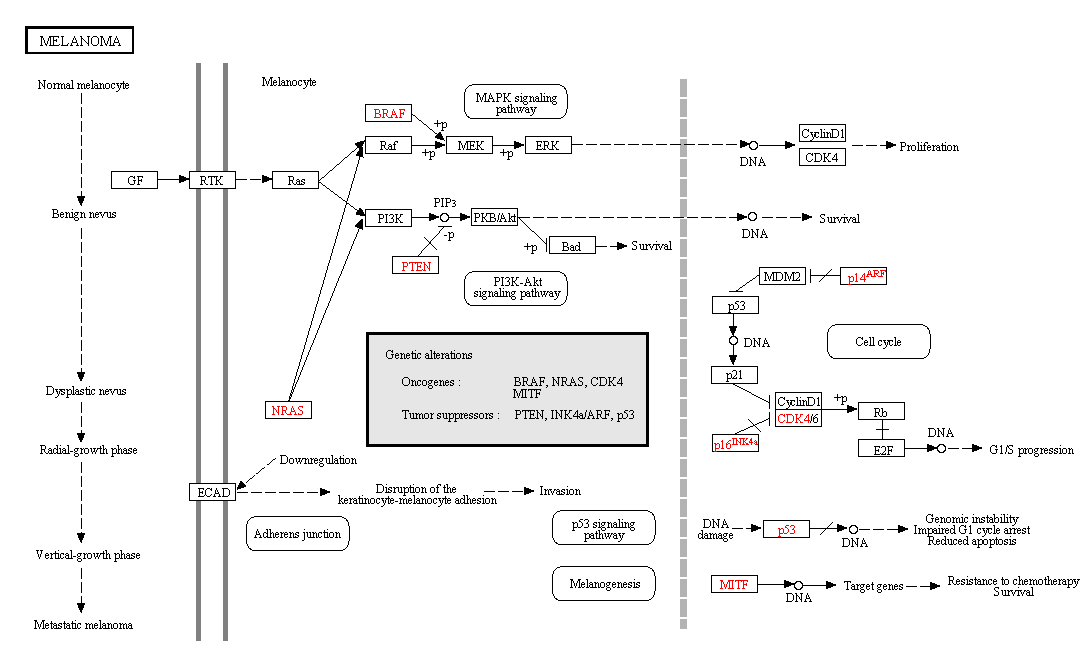
\includegraphics[width=\linewidth]{figures/kegg2}
  \caption{\label{fig:kvik} A view of a typical KEGG diagram. From~\cite{Fjukstad2014kvik}.}
\end{figure}

%\p{Pathways are very complex}

Researchers who work with pathway data are confronted with a number of challenges.
Pathway files may contain hundreds of proteins and biomolecules that participate in a variety of reactions.
In an abstract sense, reactions can be seen as state transitions with multiple inputs and outputs.
Participants --- genes, proteins, and other molecules within a cell --- can act as inputs or outputs to multiple reactions, and the relationships between reactions inherently include feedback loops.
Reactions often have an effect on other reactions, inhibiting or promoting their frequency.
These molecular activation pathways are inherently dynamic, which limits the utility of any static graph representation \cite{kitano2002systems}.
Representing complexity while also enabling researchers to see higher order patterns is a significant challenge \cite{saraiya2005visualizing}.

%\p{Pathways are useful for presentation}

Pathway diagrams can be useful for both presentation and analysis.
For presentation, pathway diagrams can contextualize a set of biological processes within a cell, and diagrams often show the location of cellular membranes in order to help provide a frame of reference for a given process.
Ideally, a pathway diagram allows a viewer to efficiently understand a complex set of biological relationships.

%\p{Pathways are useful for analysis}

While pathways may be useful for presenting and contextualizing a set of reactions, they can also be an important part of analyses in domains related to molecular biology and systems research, among others.
%\p{Domain context}

For example, molecular activation pathways are of critical importance to cancer researchers, who hope to understand --- and potentially disrupt --- malignant cycles of uncontrolled cellular growth, replication, and mediated cell death \cite{cairns2011regulation}.
Effective cancer drug development involves determining how proteins affected by a drug in turn affect important cellular pathways, and in this domain the downstream consequences of a particular drug effect are especially important \cite{luo2003targeting}.
In a separate domain, stem-cell researchers work with pathways that will precipitate a desired cellular differentiation into specific cell types \cite{reya2001stem}.

%\p{Static representations are not enough}

In the last decade, analyses that involve hundreds or thousands of genes and gene products have become common. When analyzing such large and complex data, visual representations can be essential.
Often, static representations are inadequate.
The complexity and amount of information that needs to be incorporated in given diagram can make static representations cluttered and difficult to interpret.
Thus, modern tools make careful use of user interactions and visualization techniques to allow a user to effectively explore and analyze pathway data.

%\p{Designing effective tools}

Designing effective visual analytics applications requires a detailed understanding of analysis tasks that are performed by the user.
Pathway data are often large and complex, and analysts will want to perform a variety of tasks depending on their research domain.
Tasks may be exploratory in nature, and a useful visualization of pathway data could reveal new insights to a researcher.
Tasks may also involve detailed queries or calculations of various network metrics, for example.
A comprehensive understanding of tasks performed by domain researchers in a typical analysis is essential to the design and implementation of an effective visual analytics application.

%\p{Other reviews}

%Here we perform a comprehensive analysis of tasks and requirements in an effort to design effective platforms for visual analytics of pathway data.
%Previous reviews of pathway analysis tools~\cite{Gehlenborg2010omics,Suderman2007tools} have surveyed the population of available applications.
%However, the most recent review was published over five years ago, and it includes only a surface-level discussion of tasks, requirements, and visual encoding techniques.

%\p{In this work}

In this work, we present a description and analysis of tasks and requirements related to biological pathway research.
Tasks were gathered from several interviews with domain experts who work with biological pathway data.
After an introduction to the structure and content of pathway data, we describe the tasks that were garnered from our interviews.
%Using these tasks, we then describe the high-level requirements of an effective visual analytics platform for pathway data.
We then review visual representations of pathway data in the context of our requirements.
We also review existing tools that implement those visual representations.
Finally, avenues of future research are considered, along with a brief summary of lessons learned from domain experts.

\subsection{Pathway data}

In order to aid an understanding of pathway visualization tools, an understanding of the structure of pathway data structures is necessary.
In this section we briefly explain the structure of typical pathway data files. 

\subsubsection{Pathway Data Model}

Information stored in any pathway data file can generally be broken down into three components:

\begin{itemize}

\item \textbf{Entity}\\
An entity is a component of a pathway such as a gene, a gene product (i.e. a protein), a complex of proteins, or a small biomolecule within a cell.
Entities are identified by name and are involved in one or more relationships.
Importantly, pathways themselves can be entities within other pathways.
\item \textbf{Relationship}\\
A relationship involves two or more entities.
Various kinds of relationships which different biological meanings are present in a pathways.
Relationships can be directed or undirected, and they can involve more than two entities (meaning the resulting network is a hyper-graph).
\item \textbf{Meta-data}\\
The complex nature of the information stored in a pathway requires additional data to be stored with each entity and relationship.
Meta-data can include experimental data, scientific information such as the molecular structure of a chemical compound, as well as links to additional resources or publications related to an entity or relationship.

\end{itemize}


\subsubsection{Pathway Data Formats}

Pathway data can be stored in one of several file formats.
In particular \textit{BioPAX}~\cite{demir2010biopax}, \textit{KEGG}~\cite{kanehisa2000kegg} and \textit{SBML} \cite{Hucka2003} are the most popular standards for storing the complex data structure described in the previous section.

These formats are XML based and represent data as an ontology. 
\emph{BioPAX}, in particular, was designed to be a general format for biological pathways across a variety of domain contexts~\cite{demir2010biopax}.
Systems Biology Graph Notation~\cite{Novere2009} is a visual standard often used to visualize \textit{BioPAX} and \textit{SBML} file formats.
Other formats are employed for the visualization of biological pathways that are not specific to the field of biology.
For instance \textit{SIF Simple Interaction Format} used by \textit{Cytoscape}~\cite{Shannon2003cytoscape} is used to visualize undirected interactions between participants.
%-------------------------------------------------------------------------
\section{Related Work}
%-------------------------------------------------------------------------
%\subsection{Biological Pathway Visualization}
%Biological networks are an important application domain and visualizations are an important tool  to understand complex biological processes.
%
%\cite{Gehlenborg2010omics}

%Previous reviews of pathway analysis tools~\cite{Gehlenborg2010omics,Suderman2007tools} have surveyed the population of available applications.
%-------------------------------------------------------------------------
\subsection{Task Taxonomies}
For some time Task taxonomies have been  used as a tool to help better understand the wide range of existing visualizations, as well as design and evaluate new systems.
Wehrend and Lewis~\cite{Wehrend1990} provide one of the earliest visualization task taxonomies, with the goal of ``accelerating progress in scientific visualization'' by allowing people to easily find the right visualization for a problem. 
Their task were, like many later taxonomies, were independent of a specific visualization application domain.
Schneiderman~\cite{Shneiderman1996} defined a task by data type taxonomy for  in formation visualization\textit{``to sort out the prototypes and guide researchers to new opportunities''}. 
This taxonomy was targeted towards information visualization in general, but later taxonomies focused specifically on different categories of visualization.  

Valiati et al. provide a taxonomy specifically dealing with multidimensional visualizations. The build on~\cite{Wehrend1990}, but focusing on tasks for multidimensional visualizations  (such as parallel coordinates).
Like previous authors their goal is to guide the choices of visualization and interaction techniques, and also to  help support usability testing.
Lee at al~\cite{Lee2006} define a graph visualization taxonomy of tasks that are frequently encountered when analyzing graph data.
The goal of this was to improve the evaluation of graph visualization systems by having common benchmark tasks (which could be used in conjunction with benchmark data sets).
The taxonomy covers graphs in general, and was inspired by example tasks from many domains as well as previous work.
The authors built on Amar and Stasko~\cite{Amar2005} low level visual analytic task list, by proposing additional ones of their own and composing higher level complex tasks from low level ones


Other more recent taxonomies focus of aspects of graph visualization.
Ahn et al~\cite{Ahn2014} provide a task taxonomy for analyzing evolving networks, also know as dynamic graphs. The dynamic nature of the graphs means tasks may be specified that are  not covered by the general graph taxonomy of lee et al.
Pretorius et al~\cite{Pretorius2014} focus on multivariate graph visualization (where graph elements contain multiple attributes) 
They build on the work  of Lee et al, but also on that of  Valiati et al as multivariate networks can be considered a multidimensional data set.


It can be seen from the preceding list that as visualization research has progressed taxonomies have become more focused on specific data types.
Biological Pathway visualization is a complex application domain. 
Previous taxonomies have avoided being domain specific, however this domain poses many specific challenges not encountered in the created of the previous taxonomies
The underlying data sets are dynamic multivariate hyper-graphs, and are more complex than any of those described in previous taxonomies.
The tasks to be completed by biologists are also highly complex, involving many different entity and relationship types, and are not fully covered by the existing taxonomies.
\todo[inline]{Need to be 100 percent sure this is true}
%Amar and stasko do include correlation as one of their tasks
% pretorius also includes causation...

%-------------------------------------------------------------------------



\section{Interviews}

%-------------------------------------------------------------------------
\section{Task Taxonomy}
\subsection{Taxonomy Overview}
\subsection{High Level Task}
%HIgh level task overview
\paragraph{Low Level Task 1}
\paragraph{Low Level Task 2}




%-------------------------------------------------------------------------
\section{Discussion}

\subsection{Future Research Directions}

\section{Conclusions}



%-------------------------------------------------------------------------

%\bibliographystyle{eg-alpha}
\bibliographystyle{eg-alpha-doi}

\bibliography{references}


\end{document}


% ---------------------------------------------------------------------
% EG author guidelines plus sample file for EG publication using LaTeX2e input
% D.Fellner, v1.17, Sep 23, 2010


\title[A Task Taxonomy to support Visualization for the Effective Analysis of Biological Pathways]%
      {A Task Taxonomy to support Visualization for the Effective Analysis of Biological Pathways}

% for anonymous conference submission please enter your SUBMISSION ID
% instead of the author's name (and leave the affiliation blank) !!
\author[]{SUBMISSION ID}

% ------------------------------------------------------------------------

% if the Editors-in-Chief have given you the data, you may uncomment
% the following five lines and insert it here
%
% \volume{27}   % the volume in which the issue will be published;
% \issue{1}     % the issue number of the publication
% \pStartPage{1}      % set starting page


%-------------------------------------------------------------------------
\begin{document}

% \teaser{
%  
\includegraphics[width=\linewidth]{eg_new}
%  \centering
%   \caption{New EG Logo}
% \label{fig:teaser}
% }

\maketitle

\begin{abstract}
Understanding complicated networks of interactions and chemical components is essential to solving contemporary problems in modern biology, especially in domains such as cancer and systems research.
In these domains, biological pathway data is used to represent chains of interactions that occur within a given biological process.
Visual representations can help researchers understand and interact with complex pathway data in a number of ways.
Biological data sets offer unique challenges for visualization, due to their complexity and heterogeneity.

Here, we present taxonomy of tasks -- generated from interviews with several domain experts -- that are regularly performed by researchers who work with biological pathway data.
These tasks require further classification than is provided by existing taxonomies.

\todo[inline]{more here about how these tasks are different from previous work}

We also examine the existing visualization techniques which support each of the tasks, and we discuss gaps in the existing visualization space revealed by our taxonomy.
We conclude by suggesting future research directions based on our taxonomy and motivated by the comments received by our domain experts.


\begin{classification} % according to http://www.acm.org/class/1998/
\CCScat{Computer Graphics}{I.3.3}{Picture/Image Generation}{Line and curve generation}
\end{classification}

\end{abstract}

%-------------------------------------------------------------------------
\section{Introduction}

Understanding complicated networks of bio-molecular interactions and chemical components is essential to solving contemporary problems in modern biology, especially in domains such as cancer and systems research~\cite{hanahan2011hallmarks}.
These bio-molecular interactions are represented in the form \emph{pathways}, which are used to describe a chain of interactions between biochemical and biological entities within a cell.
Pathways are small, curated subsets of a much larger, complex graph of interactions between molecules, and a given pathway usually represents a particular biological process that is relevant within some research context.

Pathways are modeled as entities , relationships and meta-data.
An entity is a component of a pathway such as a gene, a gene product (i.e. a protein), a complex of proteins, a small biomolecule within a cell, or even another pathway.
Relationships between entities can be directed or undirected, can involve more than two entities, and they can represent many different types of biological relationship.
Meta-data can include attributes resulting from experimental data, provenance information (links to related publications), and links to additional resources related to the entity or relationship.
% In order to limit the scope of their analyses...
For example, Figure \ref{fig:kvik} shows a typical representation of a pathway as a human-curated node-link diagram, where nodes are biological entities and edges represent interactions between them.

\begin{figure}[htb]
  \centering
  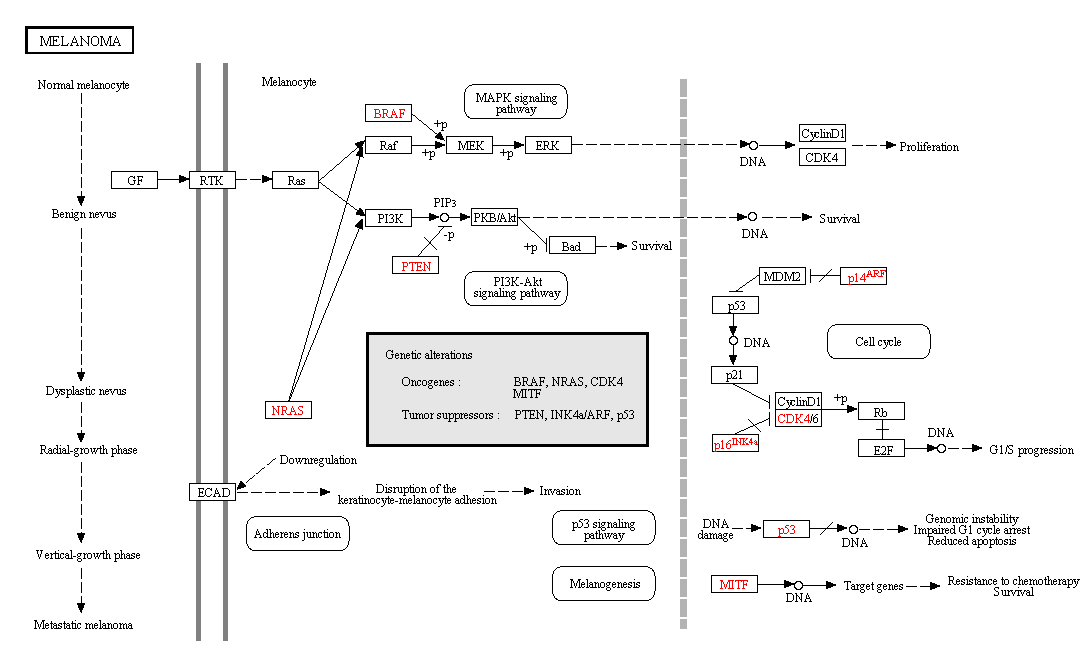
\includegraphics[width=\linewidth]{figures/kegg2}
  \caption{\label{fig:kvik} A view of a typical KEGG diagram. From~\cite{Fjukstad2014kvik}.}
\end{figure}

%\p{Pathways are very complex}

Researchers who work with pathway data are confronted with a number of challenges.
Pathway files may contain hundreds of proteins and biomolecules that participate in a variety of reactions.
In an abstract sense, reactions can be seen as state transitions with multiple inputs and outputs.
Participants --- genes, proteins, and other molecules within a cell --- can act as inputs or outputs to multiple reactions, and the relationships between reactions inherently include feedback loops.
Reactions often have an effect on other reactions, inhibiting or promoting their frequency.
These molecular activation pathways are inherently dynamic, which limits the utility of any static graph representation \cite{kitano2002systems}.
Representing complexity while also enabling researchers to see higher order patterns is a significant challenge \cite{saraiya2005visualizing}.

%\p{Pathways are useful for presentation}

Pathway diagrams can be useful for both presentation and analysis.
For presentation, pathway diagrams can contextualize a set of biological processes within a cell, and diagrams often show the location of cellular membranes in order to help provide a frame of reference for a given process.
Ideally, a pathway diagram allows a viewer to efficiently understand a complex set of biological relationships.

%\p{Pathways are useful for analysis}

While pathways may be useful for presenting and contextualizing a set of reactions, they can also be an important part of analyses in domains related to molecular biology and systems research, among others.
%\p{Domain context}

For example, molecular activation pathways are of critical importance to cancer researchers, who hope to understand --- and potentially disrupt --- malignant cycles of uncontrolled cellular growth, replication, and mediated cell death \cite{cairns2011regulation}.
Effective cancer drug development involves determining how proteins affected by a drug in turn affect important cellular pathways, and in this domain the downstream consequences of a particular drug effect are especially important \cite{luo2003targeting}.
In a separate domain, stem-cell researchers work with pathways that will precipitate a desired cellular differentiation into specific cell types \cite{reya2001stem}.

%\p{Static representations are not enough}

In the last decade, analyses that involve hundreds or thousands of genes and gene products have become common.
When analyzing such large and complex data, visual representations can be essential.
Often, static representations are inadequate.
The complexity and amount of information that needs to be incorporated in given diagram can make static representations cluttered and difficult to interpret.
Thus, modern tools make careful use of user interactions and visualization techniques to allow a user to effectively explore and analyze pathway data.

%\p{Designing effective tools}

Designing effective visual analytics applications requires a detailed understanding of analysis tasks that are performed by the user.
Pathway data are often large and complex, and analysts will want to perform a variety of tasks depending on their research domain.
Tasks may be exploratory in nature, and a useful visualization of pathway data could reveal new insights to a researcher.
Tasks may also involve detailed queries or calculations of various network metrics, for example.
A comprehensive understanding of tasks performed by domain researchers in a typical analysis is essential to the design and implementation of an effective visual analytics application.

%\p{Other reviews}

%Here we perform a comprehensive analysis of tasks and requirements in an effort to design effective platforms for visual analytics of pathway data.
%Previous reviews of pathway analysis tools~\cite{Gehlenborg2010omics,Suderman2007tools} have surveyed the population of available applications.
%However, the most recent review was published over five years ago, and it includes only a surface-level discussion of tasks, requirements, and visual encoding techniques.

%\p{In this work}

In this work, we present a description and analysis of tasks and requirements related to biological pathway research.
Tasks were gathered from several interviews with domain experts who work with biological pathway data.
After an introduction to the structure and content of pathway data, we describe the tasks that were garnered from our interviews.
%Using these tasks, we then describe the high-level requirements of an effective visual analytics platform for pathway data.
We then review visual representations of pathway data in the context of our requirements.
We also review existing tools that implement those visual representations.
Finally, avenues of future research are considered, along with a brief summary of lessons learned from domain experts.

%\subsection{Pathway data}
%
%In order to aid an understanding of pathway visualization tools, an understanding of the structure of pathway data structures is necessary.
%In this section we briefly explain the structure of typical pathway data files.
%
%\subsubsection{Pathway Data Model}
%\todo[inline, author=FMG, color=green]{Is it ok if i condense this subsubsection into a line or two and then move it with the pathway formats subsection , to the related work section?}
%
%Information stored in any pathway data file can generally be broken down into three components:
%
%\begin{itemize}
%
%\item \textbf{Entity}\\
%An entity is a component of a pathway such as a gene, a gene product (i.e. a protein), a complex of proteins, or a small biomolecule within a cell.
%Entities are identified by name and are involved in one or more relationships.
%Importantly, pathways themselves can be entities within other pathways.
%\item \textbf{Relationship}\\
%A relationship involves two or more entities.
%Various kinds of relationships which different biological meanings are present in a pathways.
%Relationships can be directed or undirected, and they can involve more than two entities (meaning the resulting network is a hyper-graph).
%\item \textbf{Meta-data}\\
%The complex nature of the information stored in a pathway requires additional data to be stored with each entity and relationship.
%Meta-data can include experimental data, scientific information such as the molecular structure of a chemical compound, as well as links to additional resources or publications related to an entity or relationship.
%
%\end{itemize}



%-------------------------------------------------------------------------
\section{Related Work}
%-------------------------------------------------------------------------
\subsection{Biological Pathway Visualization}
%\todo[inline]{Need more here on history and importance}


%High throughput techniques have resulted in experiments producing vast amounts of highly complex data.
Pathways models are an important concept with biological research~\cite{cairns2011regulation, luo2003targeting,reya2001stem}.
The complexity of the data and the benefits offered to researchers by visualization tools make biological pathways an important application domain for visualization.


There are a large number of tools available and many existing surveys describe them \cite{Suderman2007tools,pavlopoulos2008survey,Gehlenborg2010omics}.
In this paper we highlight examples of prominent existing tools and techniques which provide support for the tasks described in our taxonomy, however it is not intended as a complete survey of biological visualization applications.
We have included the following: \textit{ChiBe}~\cite{Babur2010chibe}, \textit{Entourage}~\cite{Lex2013entourage}, \textit{Reactome Pathway Browser}~\cite{croft2014reactome}, \textit{VisAnt}~\cite{hu2004visant}, \textit{MetaViz}~\cite{bourqui2007metabolic}, \textit{VitaPad}~\cite{holford2005vitapad}, and \textit{BioFabric}~\cite{Longabaugh2012biofabric}.
It is clear from the relationship structure of pathway data that graphs are a suitable visualization choice, and each of these applications visualizes pathway data as node-link graph representations (or a slight variant in the case of Biofabric~\cite{Longabaugh2012biofabric}.
However, there are alternative visualization techniques which could be applied to pathway data.
Research has shown that matrix visualization techniques outperform node-link diagrams for higher level group based tasks\cite{Ghoniem2004,Henry2007}.
While matrix tasks are not as effective for path-tracing tasks, a juxtaposition of both types or a hybrid visualization hybrid, such as NodeTrix~\cite{NodeTrix2007}, could prove effective.
Set visualisation




\subsubsection{Pathway Data Formats}
Pathway data can be stored in one of several file formats.
In particular, \textit{BioPAX}~\cite{demir2010biopax}, \textit{KEGG}~\cite{kanehisa2000kegg} and \textit{SBML} \cite{Hucka2003} are the most popular standards for storing the complex data structures described in the previous section.

These formats are XML-based and represent data as an ontology.
\emph{BioPAX}, in particular, was designed to be a general format for biological pathways across a variety of domain contexts~\cite{demir2010biopax}.
Systems Biology Graph Notation~\cite{Novere2009} is a visual standard often used to visualize \textit{BioPAX} and \textit{SBML} file formats.
Other formats are employed for the visualization of biological pathways that are not specific to the field of biology.
For instance \textit{SIF Simple Interaction Format} used by \textit{Cytoscape}~\cite{Shannon2003cytoscape} is used to visualize undirected interactions between participants.

%However, the most recent review was published over five years ago, and it includes only a surface-level discussion of tasks, requirements, and visual encoding techniques.



%-------------------------------------------------------------------------
\subsection{Task Taxonomies}
The field of visual analytics has produced a number of \textit{task taxonomies}, which are written in an effort to understand exactly how various analytics tasks are enabled by different visualization techniques, and vice-versa.
These taxonomies help clarify the utility of existing techniques while also providing a low level template for the design and evaluation of new techniques.
Wehrend and Lewis~\cite{Wehrend1990} provide one of the earliest visualization task taxonomies, with the goal of ``accelerating progress in scientific visualization'' by allowing researchers to easily find the right visualization technique for a given problem.
Schneiderman~\cite{Shneiderman1996} define a ``task by data type taxonomy'' for information visualization in order to \textit{``to sort out the prototypes and guide researchers to new opportunities''}.
These seminal taxonomies were, like many later taxonomies, independent of a specific visualization application domain, their purpose was to provide a low level description and categorization of the analysis tasks enabled by \textit{any} visualization of data.

Later taxonomies focus specifically on more narrow categories of visualization.
For instance, Valiati et al.~\cite{Valiati2006} provide a taxonomy focused specifically on multidimensional visualizations. They build on~\cite{Wehrend1990}, but focus on tasks uniquely related to multidimensional visualizations (such as parallel coordinates).
Like previous authors, their goal is to guide the choices of visualization and interaction techniques, and also to  help support usability testing.
Lee at al~\cite{Lee2006} define a graph visualization taxonomy of tasks that are frequently encountered when analyzing graph data.
The stated goal of this work was to improve the evaluation of graph visualization systems by creating a set of common benchmark tasks (which could be used in conjunction with benchmark data sets).
Their taxonomy covers tasks for the analysis of graphs in general, and was inspired by example tasks from many domains that make regular use of graph data.
The authors build on Amar and Stasko's~\cite{Amar2005} low level visual analytic task list by composing existing low level tasks into higher level complex tasks while also proposing additional tasks that are not captured by low level tasks presented in existing taxonomies.


Several recent taxonomies focus on aspects of graph visualization that extend the work of Lee at al~\cite{Lee2006}.
Ahn et al~\cite{Ahn2014} provide a task taxonomy for analyzing networks that evolve over time, also known as dynamic graphs.
The dynamic and complex nature of dynamic graph data yields a similarly complex set of analysis tasks, and many of these tasks are not covered by the general graph taxonomy of Lee at al~\cite{Lee2006} -- thus, new tasks need to be specified.
Pretorius et al~\cite{Pretorius2014} focus on multivariate graph visualization (where graph elements contain multiple attributes).
Their work builds on the work of both Lee at al~\cite{Lee2006} and of Valiati et al.~\cite{Valiati2006}, as multivariate networks can be considered a multidimensional data set.

The earliest visualization taxonomies were written as very general classifications of low level analytic tasks related to any data visualization.
In more recent publications, and as visualization research has progressed, task taxonomies have increasingly focused on more constrained subsets of tasks related to particular types of data structures.

While recently-published task taxonomies have focused on particular data structures (or for datasets with particular characteristics), to our knowledge this is the first written in the context of the domain of biological pathway analysis.

\todo[inline]{One could argue that the whole point of a taxonomy is to be general, and to ignore domain. We should highlight the benefits of writing a taxonomy based on domain-specific tasks. Or how this interesting... etc.}

Biological Pathway visualization is a complex application domain that poses many specific challenges not encountered in the created of the previous taxonomies
The underlying data sets are dynamic multivariate hyper-graphs, and are more complex than any of those described in previous taxonomies.
The tasks to be completed by biologists are also highly complex, involving many different entity and relationship types, and are not fully covered by the existing taxonomies.
\todo[inline]{Need to demonstrate 100 percent that this is true in the rest of the paper}
%Amar and stasko do include correlation as one of their tasks
% pretorius also includes causation...

%-------------------------------------------------------------------------

\section{Interviews}

Interviews were conducted with seven biological scientists, each of whom works with pathway data in some form.
Those interviewed included one tenured professor, three assistant professors, one researcher at a cancer research institution, one postdoctoral research associate, and one masters student in bioinformatics.
Interviews were loosely structured, but interview questions were designed to elicit a detailed understanding of the tasks performed by the researcher in a typical analysis, as well as an understanding of the type and structure of data that each researcher worked with.
Each researcher also presented their views on the utility of pathway data and pathway diagrams in general.

%-------------------------------------------------------------------------
\section{Task Taxonomy}

\subsection{Taxonomy Overview}

Biological pathways are generally represented as weighted, directed graphs and in some cases include hyper-edges and compound nodes.
Task taxonomies have been created which describe tasks related to graphs in general. However, the analysis of biomolecular interaction networks includes a unique set of tasks that refine and extend the tasks associated with the visual analysis of networks in general.

\subsection{Attributes}

The low-level identification of nodes, vertices, and their attributes is an essential component in the visual analysis of any graph representation.

\subsubsection{Provenance}

Especially important to researchers in the field of bioinformatics is the concept of \textit{data provenance}, which refers to the history of original sources tied to a particular entity. Much of the data in the field of bioinformatics is gathered and integrated from a wide range of publications, data stores, and other products of research.

\subsubsection{Uncertainty}

Related to the task of identifying data provenance is the task of being able to view and identify information related to the \texit{uncertainty} of the data underlying relationships between entities.

In interviews, researchers discussed the importance of understanding \emph{uncertainty} within pathway data. For example, each relationship within a BioPAX file is usually associated with a publication that provides evidence for its existence. Thus, some relationships may be subject to scrutiny within the scientific community, while others may have more robust empirical support.

\subsection{Relationships}

Understanding how pathway entities are connected was of critical importance to all of the researchers we interviewed, and is essential to most research in bioinformatics.

\subsubsection{Directed Relationships}

While some analyses and datasets involve undirected relationships between genes or gene products, studies of metabolic networks and other inter-cellular processes rely on directed relationships, and several researchers that we interviewed stressed the importance of understanding directed relationships between entities.

\subsubsection{Cause and Effect AND? Cascading Effects}

\todo[inline, author=PM]{Should we separate discussion of cause and effect from discussion of cascading effects?}

\todo[inline, author=FMG]{I think it would be a good idea to differentiate this taxonomy from ahn's taxonomy in this section. He does look at causal tasks and repetition, which are related to feedback loops , but not the same....}

A category of tasks inherent to a variety of work in bioinformatics is the identification of \textit{causal relationships} that exist between bio-molecular entities.
When discussing directed paths between entities, one entity is said to be \emph{upstream} or \emph{downstream} of another.

Understanding these upstream and downstream relationships is particularly important to domains such as cancer drug research, where a drug may affect a small subset of genes or gene products, which in turn will affect various downstream processes.
\emph{Causal networks} are also particularly essential to the analysis of large-scale gene expression data.
For instance, a causal network could reveal the likely regulators of a set of genes that are observed to be up-regulated or down-regulated in a particular setting~\cite{felciano2013predictive, Kramer2013ipa-causal}.

In most cases, a directed relationship is meant to represent a biochemical reaction, where one entity is consumed as a reactant and another is produced as a product.
Thus, an upstream entity may be connected to a downstream entity through a chain of several directed links.
In the most basic sense, the ``entities'' mentioned above are genes, gene products (such as proteins or complexes), or other small molecules within a cell.
A researcher may be interested in understanding the path of reactions (or other relationships) that connects two entities.

\subsubsection{Compound Relationships}

A vertex that contains other entities can be represented as a \textit{compound node}, which is equivalent to a ``parent'' vertex or in some contexts a ``module.''

It is important to note that a one-to-one relationship between an entity and a parent is \textit{not} the same as a one-to-many relationship between an entity and all of that parents children.
For instance, BioPax data contains the abstract ``NextStep'' relationship, which defines, as the name suggests, an arbitrary notion of the ``next step'' of some biological process.
A biochemical reaction could be connected, via a \textit{single} ``NextStep'' relationship, to an entire pathway, which could potentially contain thousands of nodes.
This relationship is clearly not the same as a biochemical reaction being connected to every entity within a pathway.

\subsubsection{Hierarchical AND/OR Structural Relationships}

Pathway data is inherently hierarchical.
Hierarchical relationships describe relationships of containment, and these relationships can be abstract or based on real biochemical interactions within a cell.
For example, a pathway (itself an abstraction) can be nested within other pathways.
These nested pathways generally encapsulate some commonly-understood hierarchy of biological processes that take place within a cell, such as cellular replication.
Other representations include the more general notion of a ``module'' of connected components, such as gene products.
Hierarchical relationships can also represent physical interactions between biochemical participants.
A common of example of this is in bio-molecular complexes, which are themselves composed of other complexes or biomolecules.

It is important to note that hierarchy and ``structure'' often co-exists with other types of relationships. In most cases, pathway data includes relationships of hierarchy (i.e., when one vertex is contained within another) \textit{in parallel} with other, non-hierarchical relationships, such as the relationship between one gene product that activates or inhibits another. Also, note that while non-hierarchical relationships can take a variety of forms, the only form of hierarchical relationship is one of \textit{containment}, from parent to child, and is undirected.

\subsubsection{Feedback Loops}

Feedback loops are common within metabolic activation networks, and they play a key role in processes related to uncontrolled cellular growth in cancerous cells.

\subsection{Comparisons}

\subsection{View Multiple Datasets}
\todo[inline, author=FMG]{Could this be considered a comparison task? ( where viewing multiple data sets is the solution}

\subsection{Rename: Comparing Networks to each other}

\subsection{Modification and Curation}

Several of the researchers mentioned certain tasks related to the curation, maintenance, and understanding of pathway data.

Several of the researchers mentioned certain tasks related to the curation, maintenance, and understanding of pathway data. For instance, one researcher mentioned the importance of being able to \emph{debug} potentially flawed data. Two others expressed a need to create ``personalized'' pathways that only include a user-determined subset of entities and relationships.

%-------------------------------------------------------------------------

% RG mentioned the importance of being able to \emph{debug} potentially flawed data. NH and FZ both expressed a need to create ``personalized'' pathways that only include a user-determined subset of entities and relationships.

% \todo[inline, author=FMG]{The notion of data provenance  (which publications it comes form) was very important to researchers i have talked to. It clearly relates to uncertainty visualization but maybe it could form a task in eits own right. Identify Entity provenance??}

% While in a strict sense, a hierarchical relationship between nodes can be seen as one particular type of edge, we instead explicitly distinguish between between hierarchical and non-hierarchical relationships.
% This distinction is motivated by the observation that

% \todo[inline]{need to be consistent about how we talk about compound nodes aka parent nodes aka modules}

% \subsubsection{Task: Identify Adjacency, one-to-many}
% Given an entity, find the entities that it is connected to.
%
% \subsubsection{Task: Identify Adjacency, many-to-many}
% Given a set of entities, find all other entities that are connected to that set.
%
% \subsubsection{Task: Identify Adjacency, one-to-many, outgoing}
% Given an entity, find the entities that it is connected to via outgoing edges.
%
% \subsubsection{Task: Identify Adjacency, one-to-many, incoming}
% Given an entity, find the entities that it is connected to via incoming edges.

% \subsubsection{Task: Identify Containment, parent-to-parent}
% \subsubsection{Task: Identify Containment, parent-to-leaf}
%
% \subsection{Compositions of Adjacency Tasks and Hierarchy Tasks}
% Given our distinction between hierarchical and non-hierarchical relationships, we can characterize compositions of tasks related to the identification of relationships between entities and hierarchies.
%
% These relationships occur frequently in biological pathway data.
%
% \todo[inline]{examples}

% \subsection{Relationship Task Compositions}
%
% identification of:
% \\
% \\
% relationship type: adjacency, hierarchy
% \\ $\times$
% node type: simple, compound
% \\ $\times$
% from: one, many
% \\ $\times$
% to: one, many
% \\ $\times$
% directed, undirected

% \subsubsection{Task: Identify Adjacency, parent-to-parent, one-to-one}
% \subsubsection{Task: Identify Adjacency, entity-to-parent, one-to-one}
% \subsubsection{Task: Identify Adjacency, parent-to-parent, one-to-many}
% \subsubsection{Task: Identify Adjacency, entity-to-parent, one-to-many}
% \todo[inline]{Should we further sub-divide into directed and undirected?}



% \todo[inline]{More on Activation and Inhibition? Activation and inhibition vs up-regulation and down-regulation?}

% \subsection{Cause and Effect Task Compositions}
%
% identification of:
% \\
% \\
% relationship type: increasing, decreasing, other modification
% \\ $\times$
% node type: simple, compound
% \\ $\times$
% from: one, many
% \\ $\times$
% to: one, many
% \\ $\times$
% directed, undirected

% \subsubsection{Task: Identify Cascading Effects, one-to-one}
% \subsubsection{Task: Identify Cascading Effects, one-to-many}
% \subsubsection{Task: Identify Cascading Effects, many-to-many}
% \subsubsection{Task: Identify Cascading Effects, many-to-one}

% \subsubsection{Task: Identify Feedback Loops}



% \subsection{Compound Relationships and Multiple Datasets}



% \subsection{Pathway Modification and Curation}



%-------------------------------------------------------------------------
\section{Discussion}

\subsection{Future Research Directions}

\subsection{Visualizing Uncertainty}

Especially considering our feedback from domain experts, tools generally do not attempt to visualize the ``uncertainty'' behind a connection in a pathway, as expressed by the first domain expert. This is a challenging task, as even the definition of ``uncertainty'' may be difficult to operationalize. However, data formats such as \emph{BioPAX} do have robust support for citations, allowing published references to be connected to entities and relationships within a pathway. A tool that could effectively encode ``uncertainty data'' into a visualization may be very valuable to systems researchers who work with the results of hundreds or thousands of separate publications.

\section{Conclusions}



%-------------------------------------------------------------------------

%\bibliographystyle{eg-alpha}
\bibliographystyle{eg-alpha-doi}

\bibliography{references}


\end{document}
